\renewcommand{\arraystretch}{1.5}
\begin{longtable}{
    |p{3cm}
    |p{3.5cm}
    |p{3.5cm}
    |p{3.5cm}|
}
\caption{Comparativa de cámaras para el sistema de visión artificial} 
\label{tab:cam_comparativa} \\
\hline
\textbf{Característica} & \textbf{OV2640} & \textbf{OV5640} & \textbf{Rb Pi Camera Module 3} \\
\hline
\endfirsthead

\hline
\textbf{Característica} & \textbf{OV2640} & \textbf{OV5640} & \textbf{Rb Pi Camera Module 3}\\
\hline
\endhead

\hline
\multicolumn{4}{r}{\textit{Continúa en la siguiente página}} \\
\endfoot

\hline
\endlastfoot

Resolución máxima 
    & 1600 x 1200 (UXGA) 
    & 2592 x 1944 (QSXGA) 
    & 4608 x 2592 \\ \hline

Interfaz 
    & SCCB / DVP 
    & DVP / MIPI / I2C 
    &MIPI CSI-2 (2 lanes)\\ \hline

Voltaje de operación 
    & 1.2 V (núcleo) / 2.5--3.0 V (E/S) 
    & 1.5 V (núcleo), 2.6 / 3.0 V (E/S) 
    &3.3 V (a través del conector de cámara) \\ \hline

Consumo activo 
    & 117 mA 
    & 140 mA
    &~250 mA  \\ \hline

Consumo en reposo 
    & 620\,\unit{\micro\ampere} 
    & 20\,\unit{\micro\ampere} 
    &$<$ 1 mA \\ \hline

Formato de salida 
    & 8-/10-bit RGB RAW 
    & 8-/10-bit RGB RAW 
    &12-bit RAW, JPEG, YUV420, RGB\\ \hline

Velocidad máxima de transferencia de imágenes 
    & \begin{itemize}[leftmargin=*]
        \item UXGA: 15 fps 
        \item SXGA: 15 fps 
        \item SVGA: 30 fps 
        \item CIF: 60 fps
      \end{itemize}
    & \begin{itemize}[leftmargin=*]
        \item QSXGA (2592×1944): 15 fps 
        \item 1080p: 30 fps 
        \item 1280×960: 45 fps 
        \item 720p: 60 fps 
        \item VGA (640×480): 90 fps 
        \item QVGA (320×240): 120 fps
      \end{itemize} 
    & \begin{itemize}[leftmargin=*]
        \item 4608×2592: 30 fps 
        \item 2304×1296: 60 fps 
        \item 1536×864: 120 fps
     \end{itemize}\\ \hline

Compatibilidad 
    & ESP32, STM32, Arduino, FPGA, Raspberry Pi 
    & ESP32, STM32, Arduino, FPGA, Raspberry Pi 
    & Raspberry Pi (todas las versiones con conector CSI)\\ \hline

Costo aproximado 
    & \$5--10 USD 
    & \$12--18 USD
    & \$64 USD\\ \hline

Ventajas destacadas 
    & Muy bajo consumo, compatibilidad con sistemas embebidos 
    & Alta resolución y mayor calidad de imagen 
    &Autoenfoque, HDR, excelente calidad en condiciones de baja luz\\ \hline

Imagen 
    & \shortstack{\\ 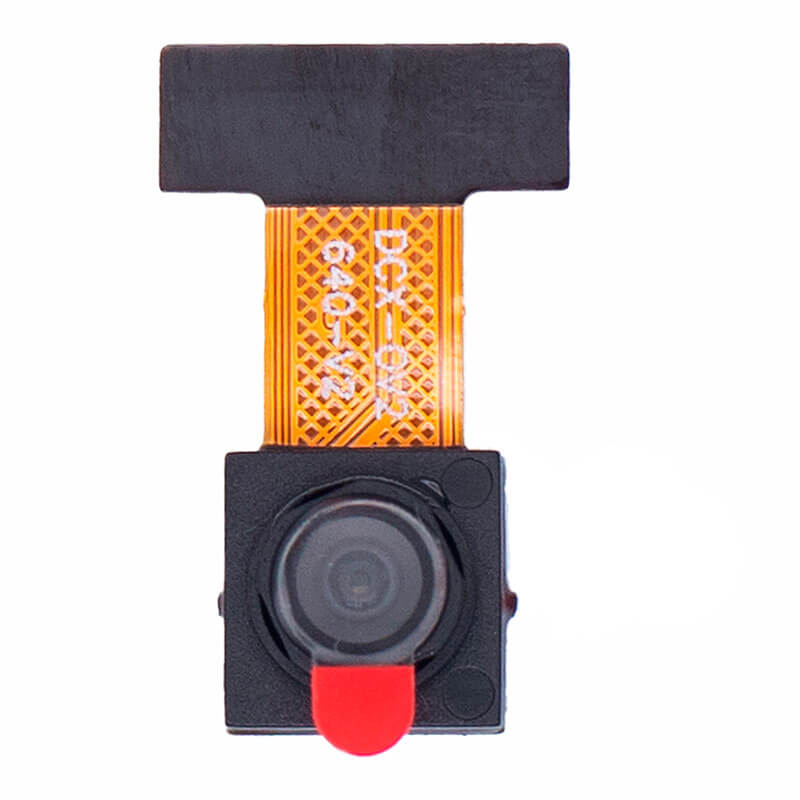
\includegraphics[width=0.6\linewidth]{Documento/Imagenes/Análisis/Cámaras/Camara-OV2640.jpg}} 
    & \shortstack{\\ 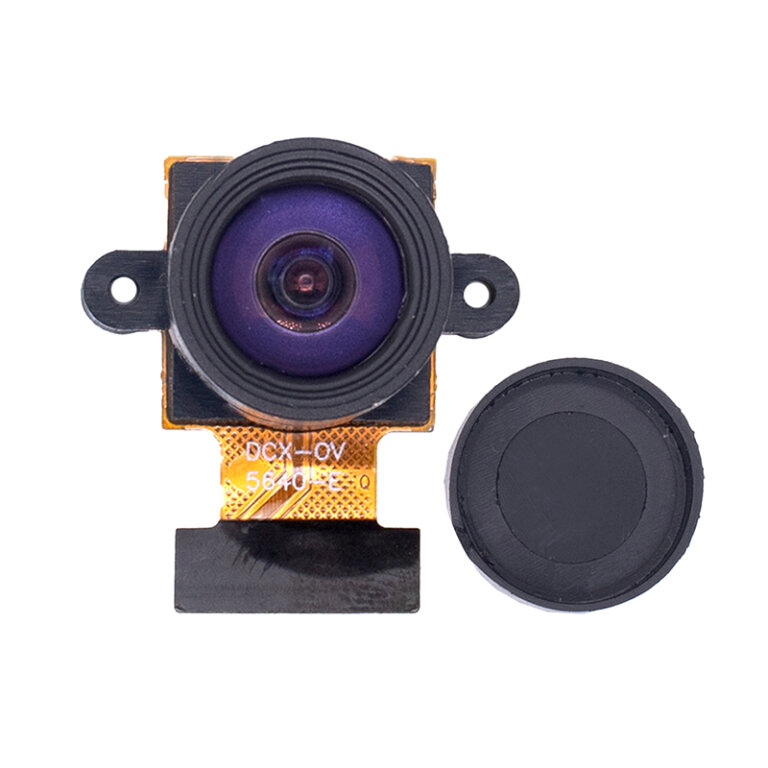
\includegraphics[width=0.6\linewidth]{Documento/Imagenes/Análisis/Cámaras/Camara-OV5640.jpg}} 
    & \shortstack{\\ 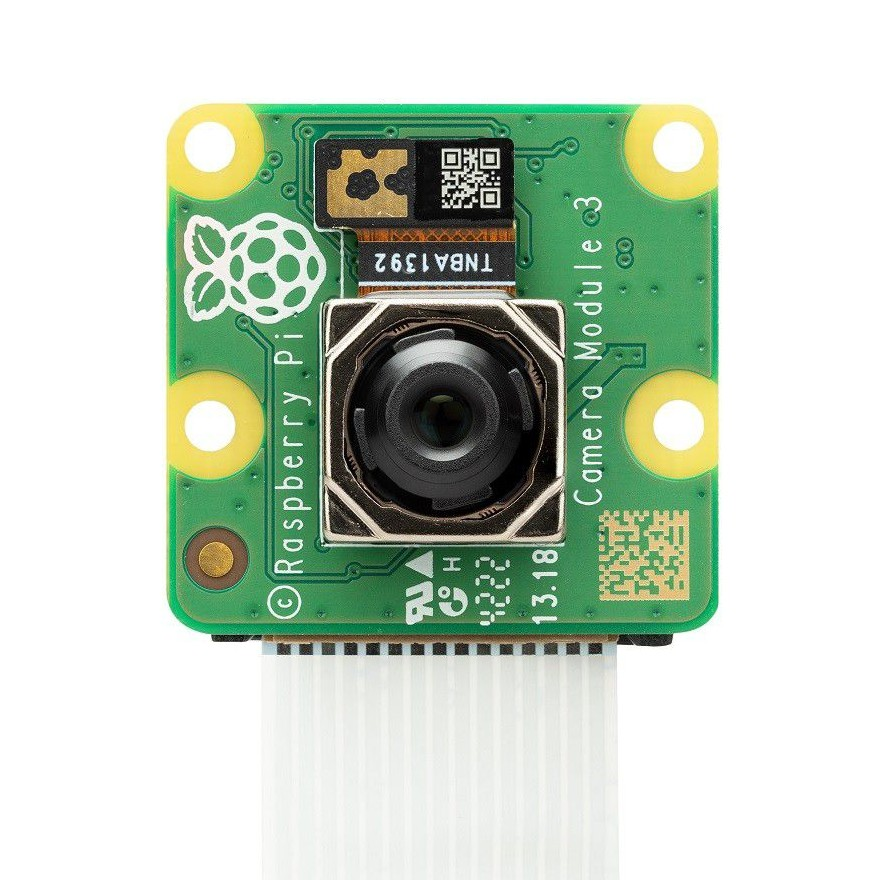
\includegraphics[width=0.6\linewidth]{Documento/Imagenes/Análisis/Cámaras/module3.jpg}} \\ \hline

\end{longtable}
